\documentclass[12pt, a4paper, oneside, parskip=full]{memoir}

\setulmarginsandblock{2.5cm}{3cm}{*} % Upper-Lower margins
\setlrmarginsandblock{3.8cm}{2.5cm}{*} % Left-Right margins
\checkandfixthelayout

%******************************
%      Table of con../fig../tab..
%*************************
\renewcommand{\contentsname}{TABLE OF CONTENTS}
\renewcommand{\listfigurename}{LIST OF FIGURES}
\renewcommand{\listtablename}{LIST OF TABLES}
\renewcommand{\printtoctitle}[1]{\centering\Large\bfseries #1}
\renewcommand{\printloftitle}[1]{\centering\Large\bfseries #1}
\renewcommand{\printlottitle}[1]{\centering\Large\bfseries #1}
\renewcommand{\chapternumberline}[1]{\MakeTextUppercase{\chaptername\ 
\numtoName{#1}: }}
\setcounter{tocdepth}{3}
\abstractintoc % Show abstract in ToC
\renewcommand\cftchaptername{\chaptername~}

\usepackage{times} % Use Times font

%******************************
%      Spacing
%*************************
\usepackage{parskip}
\setlength{\parindent}{1.2cm} % Paragraph indent
\frenchspacing % Use single space after end of sentence
\DoubleSpacing

%******************************
%      Others
%*************************
\usepackage{hyperref}

%******************************
%      Testing Only
%*************************
\usepackage{blindtext}
\usepackage{lipsum}
\usepackage[showframe, pass]{geometry} % Show page frames

\begin{document}
%******************************
\frontmatter
%*************************
\begin{abstract}
\lipsum[1]
\end{abstract}
\newpage

\tableofcontents*
\listoftables
\listoffigures

%******************************
\mainmatter
%*************************

\Blinddocument
\subsubsection{Testing Sub-Sub section}

\Blinddocument

\chapter{Introduction}\label{introduction}

Lorem ipsum \autocite{partridge2011forty} dolor sit amet, consectetur
adipisicing elit. Voluptatem quam, blanditiis, exercitationem repellat
corporis quidem consectetur quae excepturi dignissimos sequi ipsa,
beatae animi ipsam sit perspiciatis accusantium amet, facere? Rem!

\begin{figure}
\centering
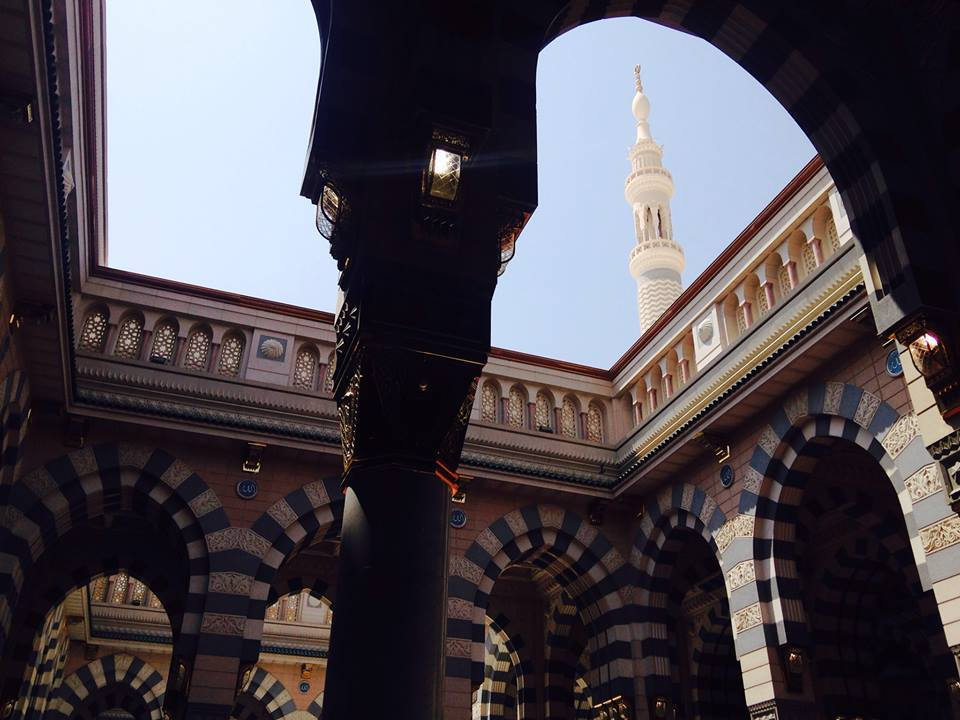
\includegraphics[width=1.00000\textwidth]{figures/madinah.jpg}
\caption{Masjid al-Nabawi, Medinah}
\end{figure}

\section{Background}\label{background}

\textcite{7282364} said Lorem ipsum dolor sit amet, consectetur
adipisicing elit. Quasi blanditiis vero placeat, aspernatur voluptatibus
reiciendis incidunt suscipit, accusamus aperiam modi, saepe quisquam
aliquam harum ipsa! Suscipit aspernatur dolorum nobis, molestiae?

\chapter{Literature Review}\label{literature-review}

Lorem ipsum dolor sit amet, consectetur adipisicing elit. Fugit
assumenda unde ex voluptatem adipisci excepturi, labore obcaecati
asperiores expedita deleniti consequuntur, sunt alias cum vero repellat
omnis earum nobis! Hic.

\section{Types of Things}\label{types-of-things}

Lorem ipsum dolor sit amet, consectetur adipisicing elit. Facilis,
similique explicabo. Architecto nam sit dolor vitae accusantium dolore
eum reprehenderit repellat debitis harum totam minus, inventore sint
corporis magni, aliquam.

\subsection{First Thing}\label{first-thing}

Lorem ipsum dolor sit amet, consectetur adipisicing elit. Laboriosam
nihil a eaque pariatur, vero nobis accusamus voluptates nulla, ipsum,
nisi enim. A cum aspernatur, repellat quo ut omnis repellendus cumque!

\subsection{Second Thing}\label{second-thing}

Lorem ipsum dolor sit amet, consectetur adipisicing elit. Laboriosam
nihil a eaque pariatur, vero nobis accusamus voluptates nulla, ipsum,
nisi enim. A cum aspernatur, repellat quo ut omnis repellendus cumque!

\subsection{Third Thing}\label{third-thing}

Lorem ipsum dolor sit amet, consectetur adipisicing elit. Laboriosam
nihil a eaque pariatur, vero nobis accusamus voluptates nulla, ipsum,
nisi enim. A cum aspernatur, repellat quo ut omnis repellendus cumque!

\subsubsection{Some Really Small Thing}\label{some-really-small-thing}

Lorem ipsum dolor sit amet, consectetur adipisicing elit. Cupiditate
eius reiciendis tempore nesciunt velit corporis totam iusto fugiat
exercitationem veritatis, sit, sint aliquid laudantium consequuntur
quasi, architecto obcaecati, ipsam facere!

\begin{longtable}[]{@{}lll@{}}
\caption{The Table's Caption}\tabularnewline
\toprule
sdasd & adasdas & sadasds\tabularnewline
\midrule
\endfirsthead
\toprule
sdasd & adasdas & sadasds\tabularnewline
\midrule
\endhead
asdasdasd & dasd & asd\tabularnewline
d & dasdas & assdasdasdasdasdasdasdasdasd\tabularnewline
\bottomrule
\end{longtable}

\chapter{Conclusion}\label{conclusion}

Lorem ipsum dolor sit amet, consectetur adipisicing elit. Doloremque,
veritatis, commodi! Ab molestiae qui modi vero dolorem quam asperiores
aliquid, quo nemo, saepe suscipit. Corrupti, saepe. Unde voluptate, sint
quasi.


%******************************
\backmatter
%*************************

\end{document}